% !TEX root = ../CSS-OS.tex

\chapter{巡天规划概要}

\GT{本章内容主要涉及巡天的目标,以及一些具体的相机参数等内容。}

\section{巡天任务指标}

巡天任务规划包括对4种观测模式的巡天任务进行规划,其中包括深度多色成像观测、极深度多色成像观测、无缝光谱观测
和深度无缝光谱观测四种。

这4种观测模式下的巡天任务指标分别为:
\begin{itemize}
\item[1.] \RT{\bf 深度多色成像观测}\\
天区面积不小于15000平方度,重点观测中高银纬($|b|\ge 20$\textdegree)、中高黄纬区域
($|\beta|\ge20$\textdegree),每一次指向的天区覆盖次数不少于2次,每次曝光时间最小150秒;
\item[2.] \RT{\bf 极深度多色成像观测}\\
在全天范围内选取多个天区观测,总面积不小于400平方度,每一次指向的天区覆盖次数不少于8次每次曝光时间最小250秒;
\item[3.] \RT{\bf 无缝光谱观测}\\
天区与深度多色成像观测天区重叠,覆盖面积不小于15000平方度,每一次指向的天区覆盖次数不少于2次,每次曝光时间最小150秒;
\item[4.] \RT{\bf 深度无缝光谱观测}\\
在深度和极深度成像观测范围内选取多个天区面积观测,观测面积不小于400平方度,每一次指向的天区覆盖次数不小于8次,
每次曝光时间最小250秒。
\end{itemize}

%\section{巡天面积}

%\section{巡天波段}

%\section{巡天深度}


\section{CCD焦面布局}

\begin{figure}[h!]
\centering
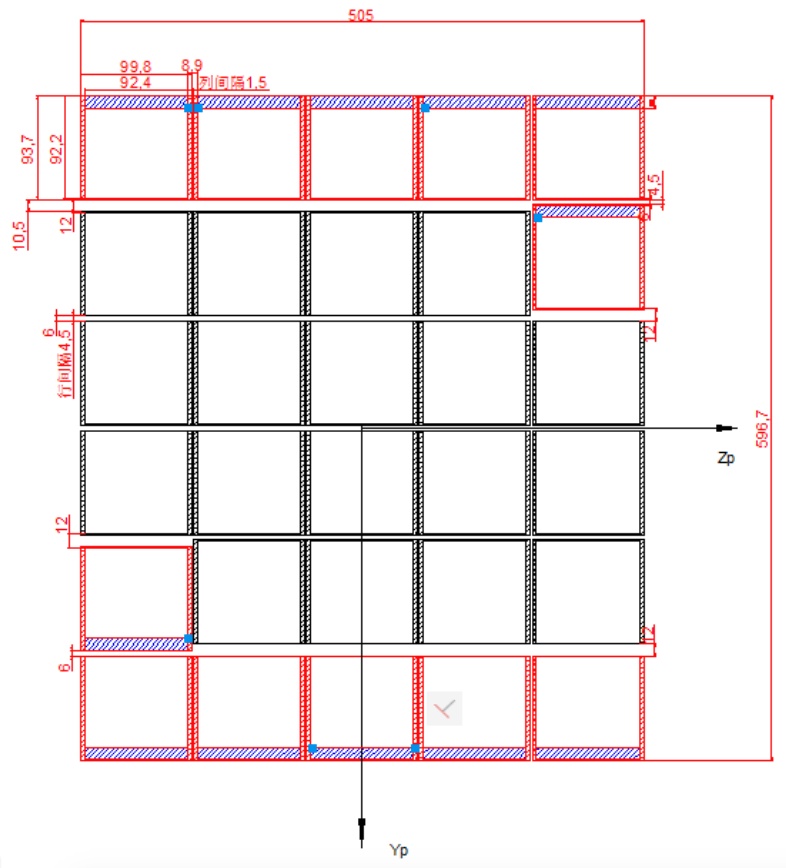
\includegraphics[width=0.65\textwidth]{figs/CCD.png}
\caption{相机CCD的布局}
\label{fig:ccd}
\end{figure}

\section{望远镜运行轨道}

\section{天区划分}
